\documentclass{article}
\usepackage[utf8]{inputenc}
\usepackage{graphicx}

\title{Research Proposal for STAT 3494W}
\author{Irene Soteriou}
\date{October 2022}

\begin{document}

\maketitle

\section*{Freedom of Speech and Physical Integrity Rights}

\section{Introduction}

For centuries, human beings have philosophized about which rights are integral to a functioning society, and which are necessary to ensure an adequate standard of living for those within it. Critical amongst these rights have been freedom of speech and physical integrity rights. Over the centuries, a plethora of literature has emerged to explore the relationship between these entitlements, from Piazza and Walsh’s ’Physical Integrity Rights and Terrorism’ to Haschke’s ’Democracy and the Human Right to the Physical Integrity of the Person.’ Many of these studies have produced divergent results with regard to the nature of this relationship, largely due to the extensive variability that exists within and between the statistical methods employed in social scientific research. Much of the diversity that exists in the existing literature can be attributed to the means by which data is collected, the differences in ways by which variables are classified, and the level of significance to which statistical results are held. Such variability makes it very difficult to draw conclusions from the existing literature about the relationship between entitlements such as freedom of speech and physical integrity rights. This presents a problem not only for the casual reader, for whom distinguishing between analyses is challenging, but also for lawmakers, policymakers, and legal and political theorists, most of whom are poorly equipped to accurately interpret the significance of these differences. Lacking the capacity to run a statistical analysis of their own, these groups are forced to resort to relying on their own limited interpretive capabilities and the opinions of advisors to craft serious governmental policies that may affect millions of people, and this weakness allows for mistakes and manipulation that may not ultimately serve the best interests of the public. While this is an issue far greater than can be addressed meaningfully by this paper, we will attempt to explore for ourselves, by rudimentary statistical analysis, the nature of any correlation, should it be found to exist, between these two fundamental rights. Doing so may give us a better understanding of the direction in which statistical analysis should go regarding social rights such as these. Moreover, such an analysis may provide insight into the true nature of the relationship in question.

\section{Specific Aims}
In this analysis, the author hypothesized that freedom of speech and physical integrity rights would be found to be positively correlated. It was anticipated that this relationship would be strong, with countries that place limits on freedom of speech exhibiting more severe infringements on physical integrity rights. The aim of this paper was to answer this question, because doing so can provide valuable insight into the ways in which societies should attempt to structure their governments and the rights provided by their legal systems so as to ensure that citizens enjoy a high quality of life. Furthermore, investigation of the aforementioned hypothesis has the potential to allow researchers to better assess negative trends in countries experiencing governmental changes, and to more astutely prevent more dangerous developments.

\section{Data Description}
The analysis conducted in this paper used as basis for investigation the CIRI Human Rights Dataset, which contains standards-based quantitative data on government adherence to numerous internationally-recognized human rights. This dataset accounts for countries of all regime-types and includes information from all regions of the world. For the purposes of this investigation, this paper compared data collected from three countries: Afghanistan, Germany, and Iran. Data was collected from 1981-2011 for each country, with 31 observations used for each of two variables: the first variable representing freedom of speech and the second representing physical integrity rights. 
The CIRI Dataset defines freedom of speech as the extent to which freedoms of speech and press are affected by government censorship, including ownership of media outlets. Censorship is defined as any form of restriction that is placed on freedom of the press, speech, or expression, and expression may be in the form of art or music. 
The CIRI Dataset defines physical integrity rights as the rights individuals have to be free from arbitrary physical harm and coercion from their government. The principal rights in this category are the rights not to be subjected to torture, political imprisonment, extrajudicial killing, and disappearance. In the CIRI index, torture is defined as “the purposeful infliction of extreme pain, whether mental or physical, by government officials or by private individuals at the instigation of government officials.” This includes the use of physical and other force by police and prison guards that is “cruel, inhuman, or degrading.” Political imprisonment refers to the incarceration of people by government officials because of their ideas, including religious beliefs; their non-violent religious practices; speech; non-violent opposition to government policies or leaders; or their membership in a group, including ethnic or racial groups. Extrajudicial killings are defined by the CIRI Dataset as killings by government officials without due process of law. This includes murders by private groups if the private actors are instigated by the government. Lastly, disappearances refer to unresolved cases in which political motivation appears likely and in which the victims have yet to be found. The CIRI dataset measures physical integrity as a five-tiered categorical variable reflective of the degree of terror, or physical integrity abuse, in a given country. The scale for this variable ranges from level 1 (no terror) to level 5 (widespread terror throughout the entire population). 
The CIRI physical integrity rights index is an empirically-verified unidimensional scale. A polychotomous extension of a probabilistic cumulative scaling technique known as the Mokken Scaling Analysis (MSA) has been used to empirically demonstrate the strong unidimensionality of the aggregated index.


\section{Methods}
To evaluate the relationship between the two variables – freedom of speech and physical integrity rights – the statistical analysis in this paper employed a simple linear regression for each of three sets of observations (Afghanistan, Germany, and Iran, all with n=31 observations). Accordingly, one simple linear regression was used to assess the strength of the relationship between freedom of speech and physical integrity rights in Afghanistan, a second simple linear regression was used to assess the strength of the relationship between these two variables as observed in Germany, and a third was used in the same manner for Iran. This approach was used to examine to what degree, if any, a relationship exists. SAS software was used to conduct this liner regression, with the independent variable for each regression being freedom of speech, coded ‘Speech,’ and the dependent variable for each regression being physical integrity rights, coded ‘PhysInt.’


\section{Results}
The SAS linear regression conducted for Afghanistan, Germany, and Iran produced intriguing results. Of the three, the data collected from Germany aligned best with the originally anticipated outcomes. As can be observed in the graph below, simple linear regression of freedom of speech and physical integrity rights revealed a strong positive correlation between the two values. However, this is really a negative linear relationship between freedom of speech and physical integrity rights, as a higher value for physical integrity rights actually correlates to more terror, which translates to a reduction in rights. So, in Afghanistan, we see that as freedom of speech increases, terror increases and physical integrity rights decreases.

\begin{figure}[htp]
    \centering
    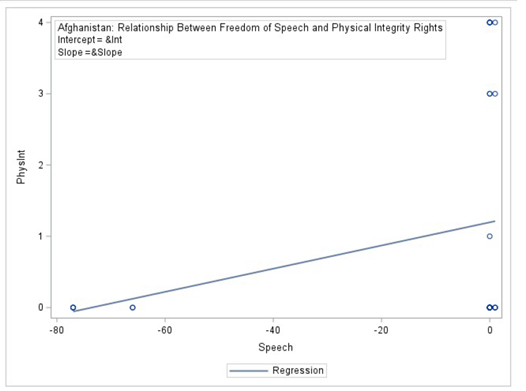
\includegraphics[width=10cm]{Afghanistan.png}
    \caption{Figure 1}
    \label{fig:Afghanistan}
\end{figure}

The same linear regression conducted for Germany revealed an outcome more aligned with that which was expected. Though the graph below shows a negative correlation between the two values, we recognize this to be a positive correlation between freedom of speech and physical integrity rights, since decreased values on the physical integrity scale correspond to less terror and thus more rights. Consequently, the analysis shows that between 1981-2011, physical integrity rights in Germany increased as freedom of speech increased.

\begin{figure}[htp]
    \centering
    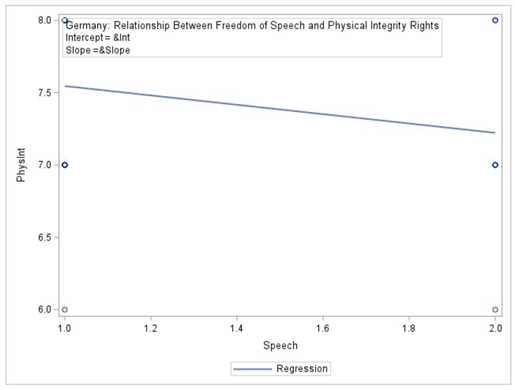
\includegraphics[width=10cm]{Germany.png}
    \caption{Figure 1}
    \label{fig:Germany}
\end{figure}

\begin{figure}[htp]
    \centering
    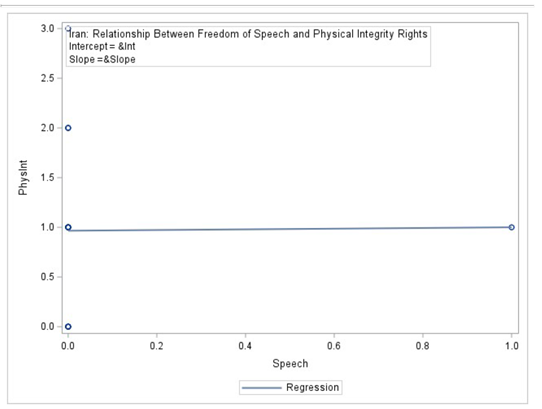
\includegraphics[width=10cm]{Iran.png}
    \caption{Figure 1}
    \label{fig:Iran}
\end{figure}

The results produced from the linear regression conducted on the data from Iran are more perplexing, as they show a very weak, if not virtually nonexistent, relationship between freedom of speech and physical integrity rights. This is illustrated below.

\section{Discussion}
At the onset of this paper, the author expected to find a strong positive correlation between freedom of speech and physical integrity rights. It seemed reasonable to suggest that restrictions on freedom of speech may often occur in countries that place greater restrictions on individual freedoms overall, and such countries tend to experience higher rates of infringement on physical rights as well. Likewise, countries that have greater freedom of speech may typically have greater infrastructure in place for public opposition to the potential for infringement on physical integrity rights. A strong positive correlation between the two variables may have been valuable to scholars and policymakers as a means of reinforcing existing assumptions about the influence and importance of freedom of speech as a means of preventing governmental tyranny and infringement of rights. Such a result is demonstrated by the outcomes of the linear regression conducted on the data collected for Germany. In the graph provided in the previous section, we see that terror decreased and physical integrity rights increased linearly as freedom of speech was expanded. 

However, the results of the investigation into Afghanistan and Iran appear to contradict these assumptions and do not match the results of Germany. In the graph of the linear regression conducted on the data collected for Afghanistan, we see a strong negative linear correlation between freedom of speech and terror (or infringement on physical integrity rights). In the graph of the regression conducted for Iran, the relationship between the two variables has a slope close to zero, suggesting that physical integrity rights are relatively unaffected by changes in freedom of speech. The varied outcomes of these three analyses are perplexing. Thus, we have reason to reevaluate our baseline principles and consider with greater scrutiny why we may be observing such results.

One thing that stands out is that for the cases in which a noticeable linear relationship does exist – namely, Afghanistan and Germany – the margins by which the dependent variable changes in response to the independent variable are relatively small. Thus, it becomes less odd for there to be very little, if any, change in the dependent variable for Iran, given that the changes observed in the dependent variable for the other two countries were already small. As for the discrepancies between the three cases, we can attempt to speculate a viable explanation as follows.

The author of this paper proposes that it may be the case that the results from the German data align with our expectations while the results from the Afghan and Iranian data do not because the data on these factors is more readily available, and more easily verifiable, in Germany than it is in Afghanistan and Iran. Germany is, by most global standards, recognized as a democratic republic with a relatively strong human rights record. Researchers can thus better collect data accurately and safely with ample opportunities to verify that data. However, both Afghanistan and Iran are internationally recognized as undemocratic countries, and their human rights records, as well as the opportunities that they have afforded researchers to collect accurate data, are poor. During the period of time during which the CIRI data was collected, it is likely that researchers would have struggled to collect accurate data from either of these nations, and the accuracy of the data may be even more poor if the numbers are based on self-reports by governing agencies. The inconsistencies in the results we see may therefore stem from inaccuracies in the data itself.

The fact remains, however, that we are nonetheless unable to explain with sufficient certainty the discrepancies in these results. This is a significant limitation in this analysis and in the data. To better investigate the potential relationship between freedom of speech and physical integrity rights, therefore, it may be more effective to conduct a similar analysis but only for data from countries where the data collected can be confirmed to be accurate to a greater degree.
Ultimately, the main contribution of the analysis in this paper is to explore a potential relationship that might be of value to the decision-making of policymakers, legal and political theorists, and all others interested in improving the structure of their societies. While the divergence in the observed results reduces the value of the conclusions that can be drawn from this analysis, our results are not entirely without significance. The existence of these discrepancies between the three countries examined indicates a need for broader analysis and points us in the direction in which we should conduct future research. We can conclude from these studies that it is important for subsequent researchers to consider the variability in accuracy of collected data which will be correlated with the countries from which these data are extracted, and that more countries must be included in analysis for that analysis to have the potential to offer more valuable results. Moreover, our results suggest that the relationship between freedom of speech and physical integrity rights may not be as clear as the author of this paper originally hypothesized, and this serves as reason to approach future research, and future policymaking, with greater care. 

Granted, the observed discrepancies between the results of the three linear analyses, as well as our lack for a confirmed explanation for this phenomenon, presents a significant limitation to the conclusions that can be drawn from this statistical analysis. No clear and consistent shared relationship can be observed to exist across the three countries, and thus we cannot conclude that a relationship does exist. Nor can we extrapolate from this analysis any conclusions about the nature of such a relationship should one exist. However, the potential explanation proposed in this paper is not without merit, and thus it provides an avenue through which future researchers may be able to better investigate, understand, and perhaps overcome, this current limitation.

\end{document}
